\chapter{Hardware}
\label{Hardware}
\section{Überblick}

Die Hardware besteht grob zusammengefasst aus den folgenden Komponenten:
\begin{itemize}
	\item Dem Longboard, bestehend aus dem Deck, den Achsen, dem Motor und der dazugehörigen Riemenübersetzung.
	\item Der Stromversorgung, die mit den Akkus dessen Kontrollschaltungen, Absicherungen und Ladeschaltung für ein zuverlässiges Handling der Energie sorgt.
	\item Der Motorsteuerung, welche die Ansteuerung des PLDC-Motors über drei Halbbrücken, einem Mikrocontroller, Strommesswiderständen und Kommunikationsschnittstellen integriert.
	\item Der Steuerung, einem Ein-Finger-Handschuh ähnlichen Konstrukt, welches die Biegung des Zeigefingers mittels eines Flex-Sensors detektiert, mit einem Mikroprozessor auswertet und über Funk dem Motorkontroller mitteilt. Ebenfalls integriert sind LED’s zur Akku-Ladestand- und Bedienanzeige sowie ein Taster zur Kalibration.
\end{itemize}
Auf die einzelnen Punkte wird in den folgenden Kapiteln noch detaillierter eingegangen. Hier wird noch kurz die Verbindung untereinander beschrieben:

Die Stromversorgung, montiert bei der nicht angetriebenen Achse, liefert die Energie über zwei Leitungen aus Kupferband zur Motorsteuerung. Das Kupferband ist Unter dem Grip-Tape versteckt, und besteht aus zwei Schichten des Bandes. Eine auf dem Brett, eine auf dem Grip-Tape, jeweils nach ca. 15cm aufgetrennt, damit durch die Federung des Boards das Band nicht zerrissen wird. Die Untere und die Obere Schicht sind verschoben aufgetrennt, sodass sie einander immer überdecken, und ein problemloser Stromfluss garantiert werden kann.

Die Strombelastbarkeit des 38mm breiten und 35um dicken Kupferbandes wurde mit der Berechnungsformel für Leiterbahnen angenähert.
Nach
\[ I = 9.6 * A^{0.68} * \Delta T ^{0.43},\] 
wo I der Strom in Ampère, A die Fläche in \(mm^2\), und \(\Delta\)T die Temperaturdifferenz in Kelvin,
ergibt sich ein Strom von I=60A bei einem Temperaturdelta von lediglich 35\(^\circ\). Da dieses Delta noch etwas höher werden darf, und so breite Leiter eher bessere Kühlverhalten aufweisen, wurde diese Näherung als ausreichend erachtet.
\todo{Link / Quelle einfügen:
[https://www.multi-circuit-boards.eu/leiterplatten-design-hilfe/oberflaeche/leiterbahn-strombelastbarkeit.html] }

Die Kommunikation zwischen Motorsteuerung und der Bedienung, dem Magic-Glove, basiert auf einer Funkverbindung auf 2.5GHz. Übermittelt wird der Wert der Biegung des Flex-Sensors in der einen Richtung, sowie der Akku-Ladestand in der Anderen. Auf die Details wird in den Kapiteln der Software eingegangen.


%
%Vielleicht könnte dieses Schema hier viel gewinnbringender eingefügt werden als im Abschnitt Grobkonzept?
%
%\begin{figure}[H]
%	\centering
%	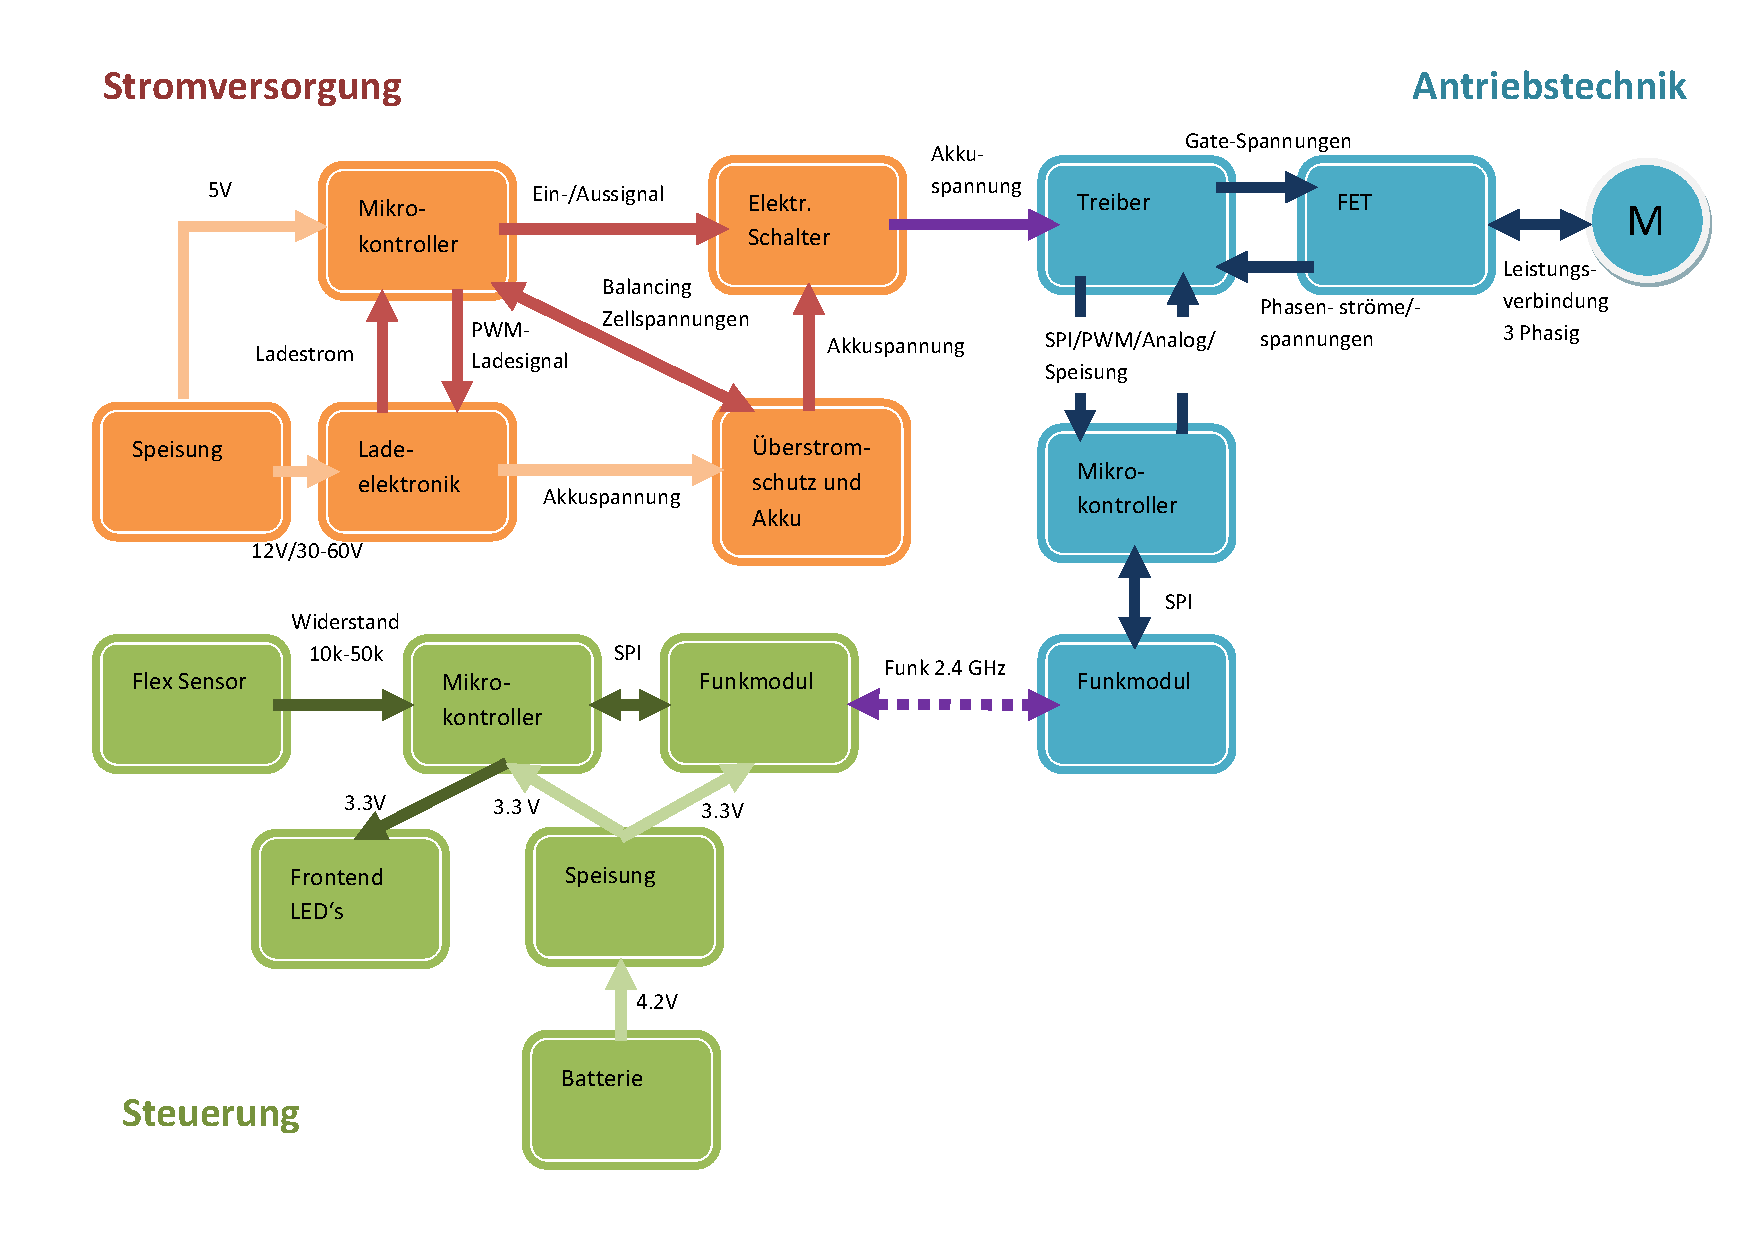
\includegraphics[width=1\linewidth]{images/Grobkonzept_Blockschaltbild_detailliert}
%	\caption[Detailliertes Blockschaltbild]{Detailliertes Blockschaltbild}
%	\label{fig:grobkonzeptblockschaltbilddetailliert_2}
%\end{figure}


\section{Steuerung - Magic-Glove}
\label{HW_MagicGlove}
Der innovative Magic-Glove ist ein Skatehandschuh der um einen Flex Sensor erweitert wurde. Somit schützt dieser bei einem Sturz nicht nur die Hände, sondern kann auch die Bewegung des Zeigefingers analysieren. Wird der Zeigefinger gestreckt, wie es beim Sturz aus Reflex passiert, wird das Board gebremst. Ballt man die Hand zur Faust, beschleunigt das Board.
Da der Flexsensor nur sehr kleine Widerstandsänderungen aufweist, wird mit der sogenannten Wheatstone-Brücke, welche in der Abbildung \ref{fig:wheatstonebruecke} zu sehen ist, gemessen.
\begin{figure} [H]
	\centering
	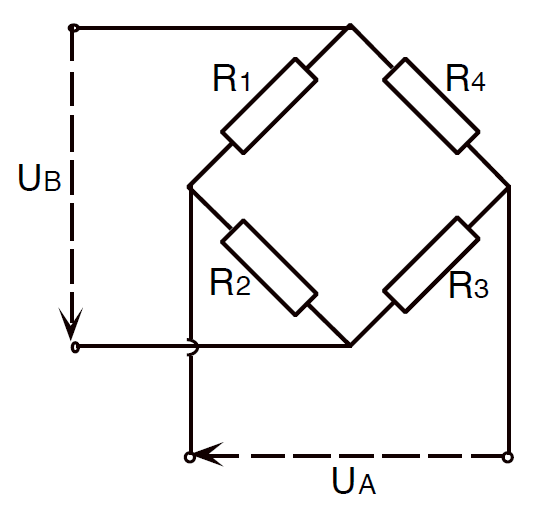
\includegraphics[width=.7\linewidth]{images/wheatstone_Bruecke}
	\caption{Wheatstone-Brücke}
	\label{fig:wheatstonebruecke}
\end{figure}
Wird eine Brückenspeisespannung $U_B$ angelegt, kann mit der folgenden Formel $U_A$ berechnet werden. 

\begin{equation}\label{glg_U_A}
 U_A=\frac{R1 \cdot R3-R2 \cdot R4}{(R1+R2) \cdot (R3+R4)} \cdot U_B 
\end{equation}
\todo{Mathe-Malpunkt suchen od ganz auslassen}
Ist der Flexsensor dabei in Ruhelage, misst man eine Spannung von 0V. Aus dem Verhältnis von $ U_A $ zu $ U_B $ erhält man die relative Dehnung S des Flexsensors \todo{Quelle Prof. Dr. Herbert Looser, „M4 Kraftmesstechnik“, FHNW, 04.06.14}.
\begin{equation}\label{S_relativeDehnung}
S=\frac{U_A}{U_B}
\end{equation}
$U_A$ wird mit dem 10-Bit Analog- Digital Wandler auf dem Mikrocontroller gemessen und mithilfe der fixen Spannung $U_B$ wird die relative Dehnung S berechnet. 


\section{Stromversorgung}
\label{HW_Stromversorgung}
An die Stromversorgung werden einige Anforderungen gestellt. So muss sie für die Motorsteuerung grosse Ströme mit bis zu 50A liefern können. Dabei muss die Spannung der Zellen kontinuierlich überprüft werden um ein Tiefentladen zu verhindern. Des Weiteren wird eine Standby-Killer Schaltung implementiert und dessen Funktion erklärt.\\
Um das Board einfach laden zu können ohne jedes Mal den Akku ausbauen zu müssen, hat sich unser Team entschieden eine Akku Ladeschaltung einzubauen. Diese muss die Zellen balancen und sie vor Überspannung bzw. Überladung schützen. 
\todo{Leserführung was kommt nun}
\subsection*{Balancing}
- ...
\subsection*{Ladeelektronik}
-	PWM zu Strom Schaltung\\
-	Selbsthaltung\\
-	Linearregler

\subsection*{Mikrocontroller}
An den Mikrocontroller werden verschiedene Anforderungen gesetzt.
In folgender Tabelle \ref{tabGPIObat} werden die General Purpose Input Output (GPIO) Anforderungen an den Mikrocontroller aufgelistet.
\begin{center}
	\begin{tabular}{|c|c|c|c|}
		\hline 
		Beschreibung & Anforderung & Input/Output & Anzahl \\ 
		\hline 
		Überwachung der Zellen & Analog & Input & 6 \\ 
		\hline 
		Überwachen des Ladestroms &	Analog & Input & 1 \\ 
		\hline 
		Überwachen der Eingangsspannung & Analog & Input & 1 \\ 
		\hline 
		&  &  &  \\ 
		\hline 
		Entladen der Zellen (Balanceing) & Digital  & Output & 6 \\ 
		\hline 
		Anzeige des Ladezustands (LED) & Digital & Output & 3 \\ 
		\hline 
		Schalten des Ausgang Stroms zum Motor & Digital & Output & 1 \\ 
		\hline 
		Selbsthaltung des Mikrocontrollers & Digital & Output & 1 \\ 
		\hline 
		&  &  &  \\ 
		\hline 
		Regelung des Ladestroms & PWM & Output & 1 \\ 
		\hline 
		Kommunikation SPI Schnittstelle MISO/MOSI/SCK & Serial & In/Output & 3 \\ 
		\hline 
	\end{tabular} 
	\captionof{table}{GPIO Anforderungen für den Mikrocontroller}
	\label{tabGPIObat}
\end{center}
Für die Regelung der Stromversorgung wird der Mikrocontroller ATmega328P-AU verwendet.
\subsection*{Zellmessung}
Die Messung der Zellen durchlief während der Entwicklungsphase mehrere Änderungen. Die Zellen sind in Serie geschaltet, um dem Motor genügend Spannung zur Verfügung zu stellen. Mit einer Zellenspannung von 4.15V pro Zelle liegt am obersten Punkt (Anode der Zelle 6) eine Spannung von 24,9V. Da die Spannung an den Eingängen des Mikrocontrollers nicht seine Speisespannung übersteigen sollte, mussten diese Spannungen verringert werden. In unserem Fall beträgt die maximale Spannung am Eingang 5V. Die erste Idee war, wie in Abb.\ref{fig:zellmessung} links oben zu sehen, mit einfachen Spannungsteiler die Spannungen so zu skalieren, dass die Maximalspannung nicht überschritten wird. 
\begin{figure} [H]
	\centering
	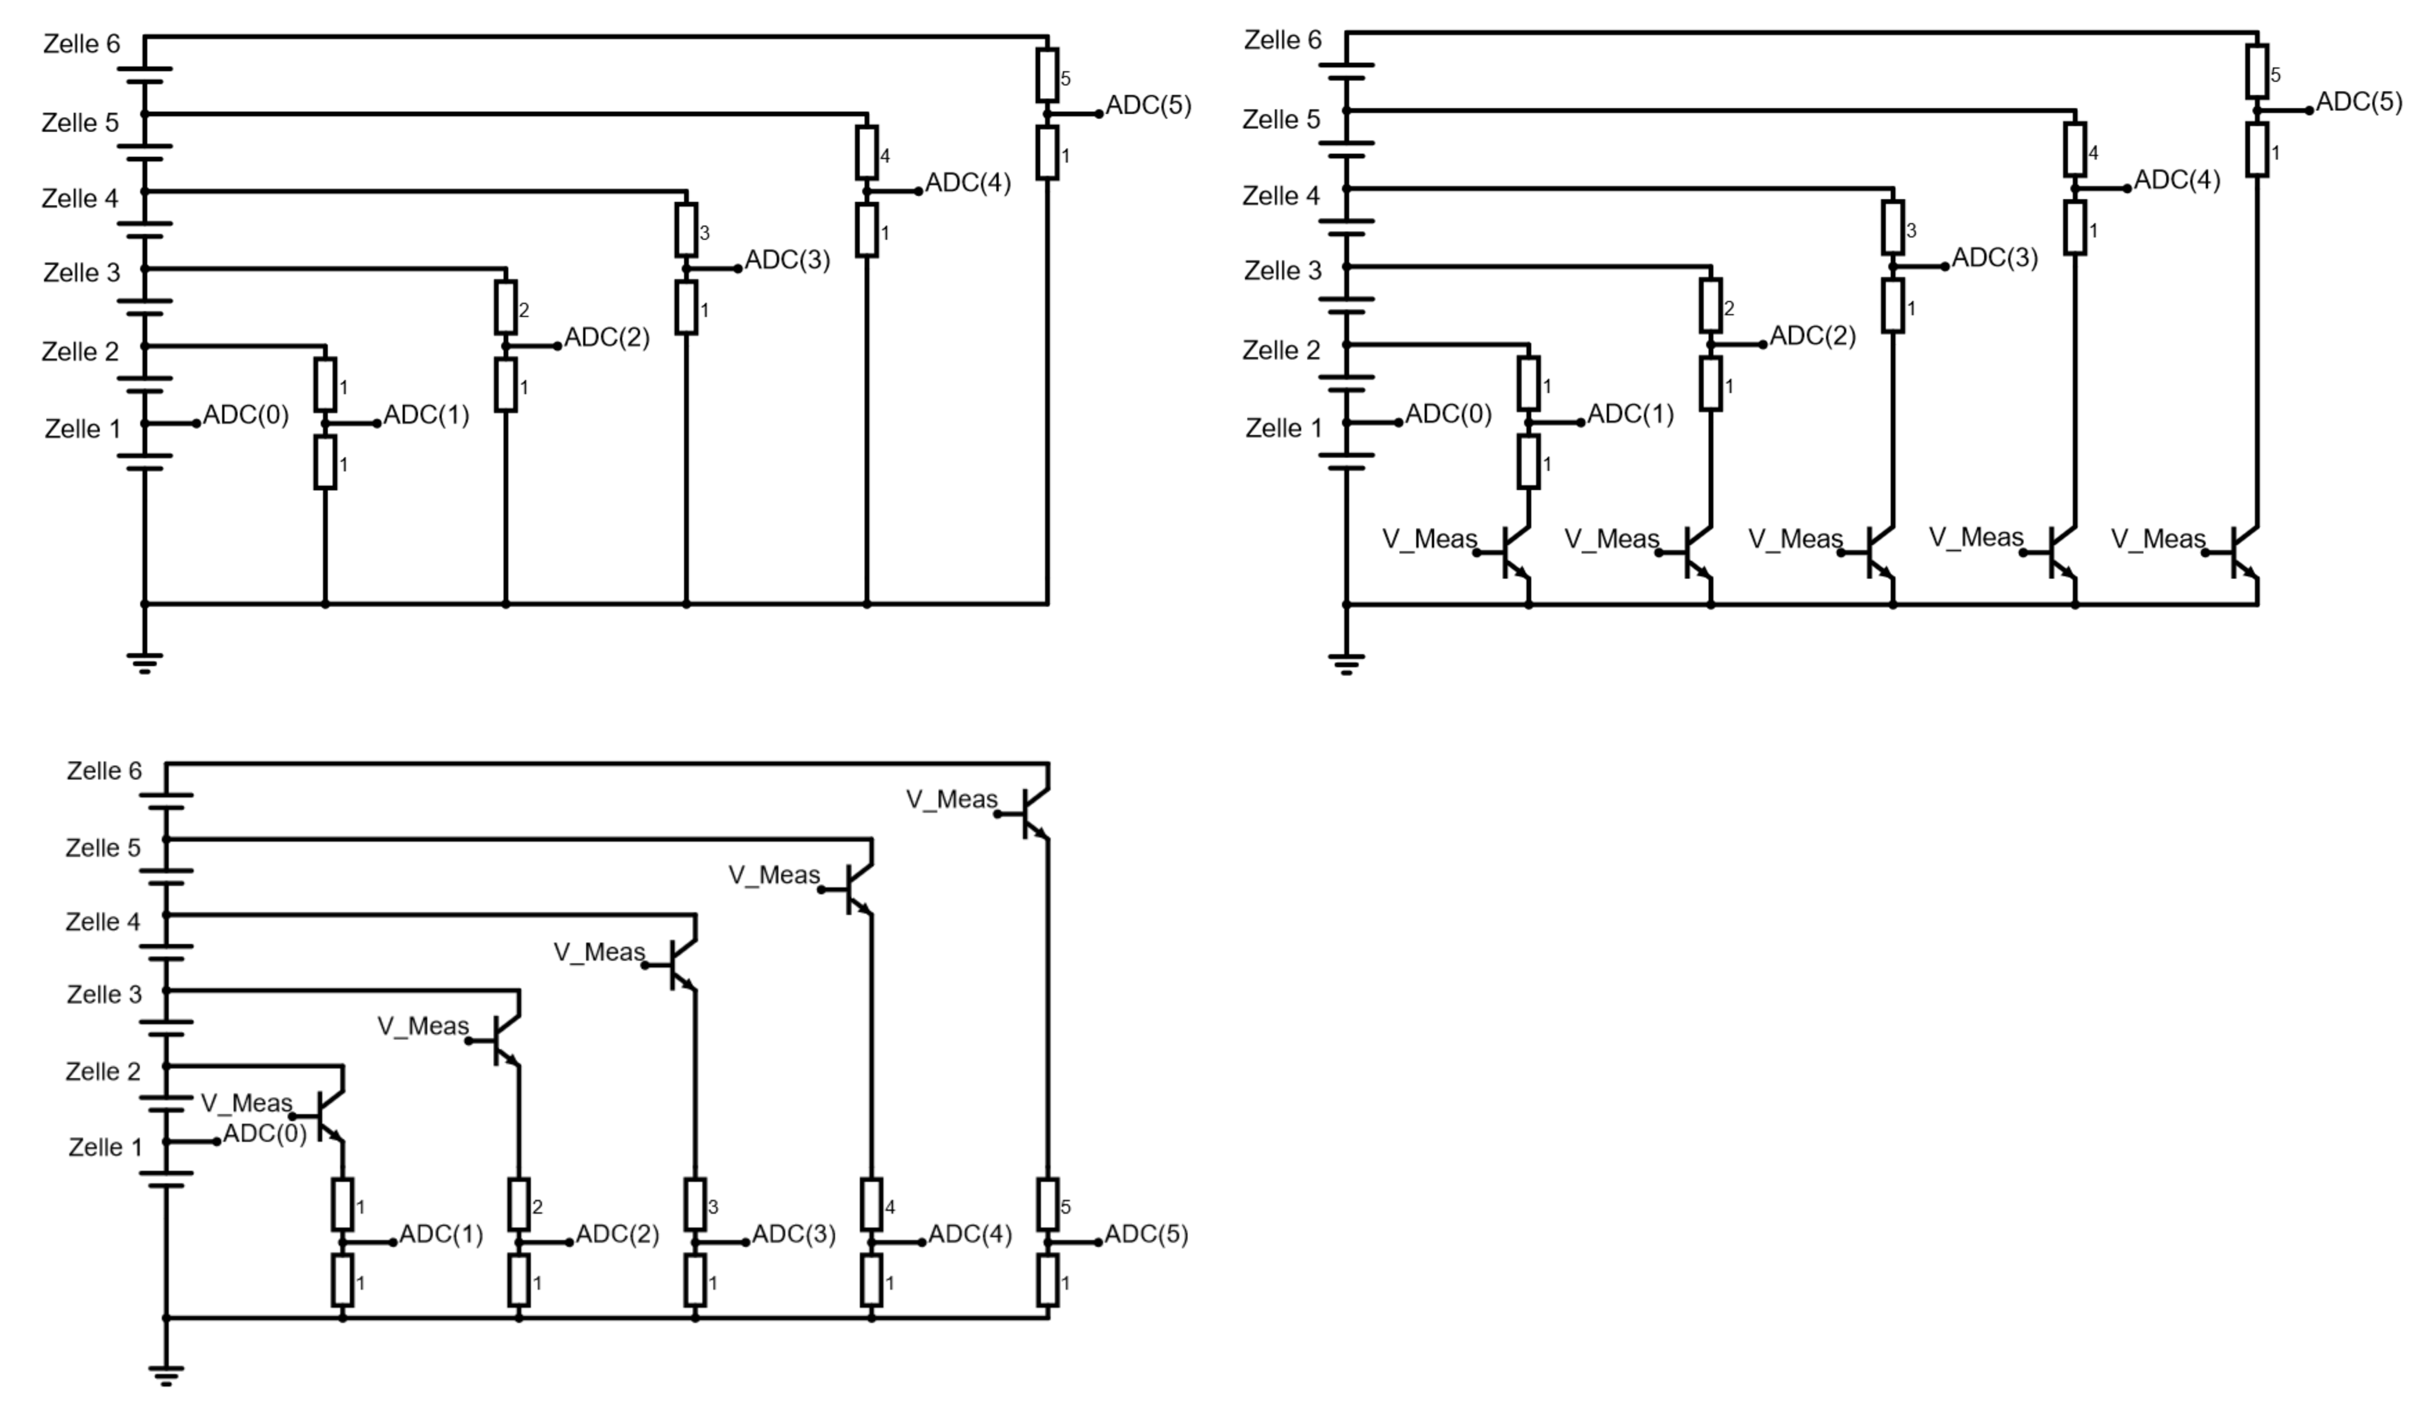
\includegraphics[width=1\linewidth]{images/Zellmessung}
	\caption{Messung der Zellen - verschiedene Arten}
	\label{fig:zellmessung}
\end{figure}
\todo{besserer Titel für Abb.}
Der Nachteil dieser Schaltung ist, dass die Zellen durch die Spannungsteiler kontinuierlich entladen werden. Somit können bei einem längeren Nichtgebrauch die Akkuzellen entladen oder sogar tiefentladen sein. \\
Um dies zu verhindern wurde der zweite Entwurf auf der rechten Seite der Abb.\ref{fig:zellmessung} entwickelt. Dieser unterbricht mit den Transistoren den Entladestromkreis über den Widerständen. Die Transistoren werden übersteuert, um sie als Schalter zu verwenden und den durch die UCE \todo{hä? bzw. Formatierung notwendig? U$_{CE}$ --> U\_collector\_emitter aaahhhaaa} Spannung entstehende Fehler zu verkleinern. Dieser tritt je nach Sättigungsspannung der Transistoren jedoch immer noch auf und ist durch die unterschiedlichen Bauarten nur schwer zu korrigieren. Der zweite grosse Nachteil und gleichzeitig Killerkriterium für diese Schaltung war, dass durch das Unterbrechen des Spannungsteiler Stromkreises an den ADC Ausgängen wieder die Zellenspannung anliegt. Dadurch würden sich die Zellen über die Ableitdiode am Eingang des Mikrocontrollers entladen und diese \todo{diese = die Ableitdiode?} voraussichtlich zerstören. \\
Dies könnte verhindert werden, indem der Stromkreis oberhalb der ADC Eingängen unterbrochen wird. Dies ist in der linken unteren Schaltung der Abb.\ref{fig:zellmessung} gezeichnet. Dadurch wären die Eingänge vor Überspannung geschützt. Aber auch diese Schaltung bringt diverse Nachteile. So fliesst beim geschlossenen Zustand der Basis-Emitter Strom durch den Spannungsteiler. Dies verfälscht die Messresultate. Zusätzlich muss zwischen Basis und Emitter eine Schaltspannung von mindestens 0.7V sein. Dazu müsste die Schaltspannung 0.7V über der Zellspannung liegen, was nur mit grossem Aufwand erreichbar wäre. 
In einem Teamentscheid wurde die erste Methode gewählt, da sie die genausten Messungen liefert und die Entladung der Zellen bei einer durchschnittlichen Benutzung des Boards nie \todo{ev.:nicht ?} zu tragen kommt.

\section{Motoransteuerung}
\label{HW_Motoransteuerung}
Die Motoransteuerung ist bei der angetriebenen Achse montiert. Bei diesem Board kommt die Drehfeldanregung mit FOC (Field Oriented Control) zum Einsatz, was bedeutet, dass die drei Phasen mit drei, jeweils um 120\(^\circ\) phasenverschobene, Sinusströmen bestromt werden. Dies erzeugt ein rotierendes Drehfeld, welches den aus Permanentmagneten bestehenden Erregerkreis auf dem Rotor in Bewegung setzt. Dieser grundsätzliche Ablauf wird hardwaretechnisch so umgesetzt:
In einem Mikrokontroller, wird pro Motorphase ein PWM-Signal erzeugt, welches integriert und gemittelt ein Sinussignal ergibt. Über einen intelligenten und schnellen Treiber werden dann die in einer H-Brücke angeordneten N-Kanal MOSFET Transistoren angesteuert, welche dieses PWM-Signal dann mit grosser Leistung an die Klemmen geben. Da jede Phase im Motor eine Spule ist, und der Strom durch eine Spule das Integral der Spannung ist, ergibt sich so dieser quasi-sinusförmige Stromverlauf.
An zwei Phasen werden die Ströme über Shunt-Messwiderstände gemessen und dem Mikrokontroller über einen A/D-Wandler mitgeteilt. Dies ist dann die Grundlage für die integrierte Regelung.

\subsection*{Mikrokontroller}
Verwendet wird der Mikrokontroller STM32F303, dies weil es ein bewährter und bekannter Mikrokontroller ist, der mit seinen 8MHz Taktfrequenz genügend schnell ist. Dazu unterstützt er die PWM Funktion, hat genügend I/O-Ports und bleibt preislich im Budget.
An ihm wird über ein SPI Interface noch das HopeRF RFM75 Modul angeschlossen, welches mit der Steuerung, dem Magic-Glove, über eine 2.5GHz Funkverbindung kommuniziert.

\subsection*{Endstufe (H-Brücken)}
Für die Ansteuerung Transistoren wird der DRV8301 Gate-Treiber von Texas Instruments verwendet. Dieser Treiber beinhaltet einen Gate Driver mit 1.7A Peak Gatestrom, Current Shunt Differenzverstärker, Über- und Unterschutzspannung sowie Übertemperaturschutz und Überstromschutz. Ebenfalls ist ein Buck Converter für die Spannungsversorgung eingebaut.
Die Transistoren sind IRFS7534 N-Kanal Power MOSFETs von Infineon, die 60V und 164A permanent aushalten. Sie eignen sich besonders für schnelles Schalten von grossen Lasten, also genau dieses Einsatzgebiet. Dies vor Allem wegen dem tiefen RDSon (typ. 2\(\Omega\)) und der geringen Eigenkapazität. 

\subsection*{Messschaltungen}
In der Ansteuerung von zwei Phasen sind 0.1\(\Omega\) Shunt-Widerstände zur Strommessung eingebaut. Die Spannung über den Widerständen wird im Gate-Treiber um den Faktor 10 verstärkt und mit einem Offset von Vlogic/2 versehen. Der Mikrocontroller erhält dann eine Spannung zwischen 0 und Vlogic von dem Treiber. Damit wird dann der Dritte Phasenstrom berechnet und dann zur Regelung verwendet.


\subsection*{Treiber IC und Speisung}
\subsection*{Endstufe (H-Brücke)}
\subsection*{Messschaltung}
\subsection*{Mikrocontroller}

